
\documentclass[a4paper,11pt]{article}

\usepackage[utf8]{inputenc}
\usepackage[T1]{fontenc}
\usepackage{tikz}            % Pretty picturessss
\usetikzlibrary{positioning} % Mah nodes need GPS
\usetikzlibrary{calc}        % Whaaat ? Math in tikz ? Is this real life ?

\begin{document}

% ==================== title ====================
\title{Rapport de projet}
\author{Alexis Laouar, Rémi Oudin, Kévin Le Run}
\date{}
\maketitle
% ===============================================

\section{Vue d'ensemble}

L'architecture du moteur de jeu est une variante du Modèle-Vue-Contrôleur où les
modèles ne sont pas purs et ont une certaine part de contrôle.

% ==================== m-v-c figure ====================
\begin{figure}[h]
  \centering
  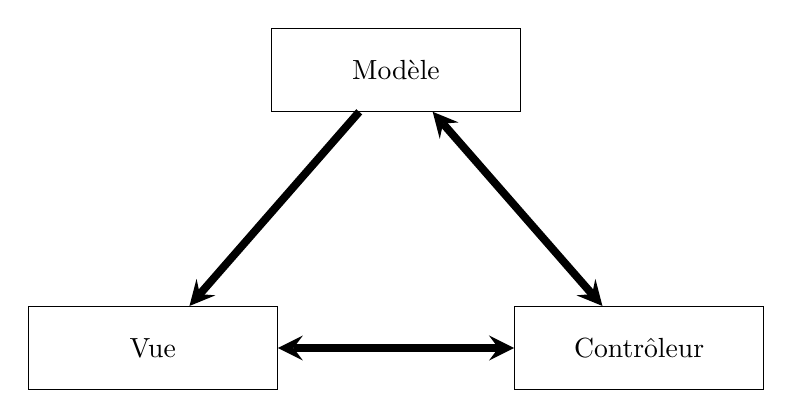
\begin{tikzpicture}[
      elementblock/.style={draw,rectangle,minimum height=3em, minimum width=9em},
      node distance=3cm]
    % Blocks
    \node[elementblock]                                     (view)      {Vue};
    \node[elementblock,right=of view]                       (controller){Contrôleur};
    \node[elementblock,above=of {$(view)!0.5!(controller)$}](model)     {Modèle};

    % Arrows
    \draw[         -{stealth},thick,line width=0.1cm] (model) edge (view);
    \draw[{stealth}-{stealth},thick,line width=0.1cm] (model) edge (controller) (controller) edge (view);

  \end{tikzpicture}
  \caption{Modèle-Vue-Contrôleur}
\end{figure}
% ======================================================

Les contrôleurs sont placés dans le package \texttt{runtime}, les modèles dans
le package \texttt{game\_mechanics} et les vues dans le package \texttt{gui}.

\section{Les contrôleurs}

Le contrôleur principal est l'objet \texttt{Controller}. Il contient la boucle
\texttt{update}-\texttt{render} ainsi que l'ensemble des modèles actifs :
les tours, les ennemis et les projectiles. À chaque tour de boucle, tous ces
modèles sont mis à jour et dessinés à l'écran. La mise à jour des mouvements se
fait par méthode d'Euler (plus de détails en section \ref{models}).

% Needs more stuff in here :)

\section{Modèles} \label{models}

Pour les modèles, nous avons distingués 3 modèles principaux.

\subsection{Les ennemis}
Les ennemis, qui possèdent leur chemin et vont principalement avancer en
recalculant la trajectoire au dur et à mesure, à l'aide de la méthode d'Euler.
Les ennemis ont les attributs suivants:
\begin{itemize}
    \item HP, qui représente leurs points de vie
    \item Shield, qui représente la réduction de dégâts
    \item Speed, qui représente leur vitesse de déplacement
    \item Reward, la récompense.
\end{itemize}

Pour bouger, l'ennemi connaît la position de la case suivante dans laquelle il
doit aller. Le mouvement qu'il effectue est continu, c'est-à-dire qu'il va de case
en case mais de manière continue, ce qui l'amène à devoir recalculer son moouvement
à chaque nouvelle case atteinte. Pour l'instant, il n'a besoin que de sa case de
départ (pour l'apparition) et de sa case d'arrivée.\\
À chaque mise à jour par le contrôleur, les monstres vérifient leur nombre de HP,
et demandent au contrôleur de l'oublier s'ils atteignent un nombre de HP négatif.

\subsection{Les tours}

Une tour a une position fixe, et diverses caractéristiques, dont la portée, les
dégâts, le coût, et le cooldown. Pour tirer, la tour prend à chaque nouveau tir
l'ennemi qui est le plus avancé vers le core, et crée un objet projectile dont
la cible est le l'ennemi visé. Il transmet les propriétés de dégâts et de vitesse
du projectile à celui-ci.

\subsection{Les projectiles}

Un projectile est un objet créé par une tour. Il a pour attributs:
\begin{itemize}
    \item Une cible qui est un ennemi,
    \item une vitesse,
    \item une position courante,
    \item des dégâts.
\end{itemize}

Il suit son ennemi, c'est-à-dire qu'à chaque étape, il va récupérer la position
courante de sa cible, et se diriger vers lui. On considère que si après avoir bougé,
un projectile a dépassé sa cible, il l'a touché. Alors, le projectile demande à
sa cible de se retirer des HP.

\section{Vues}

% TODO

\section{Conclusion} % Maybe ?

% TODO

\end{document}
